\chapter{CT Fourier Transform}

Recall the complex exponential $e^{st}$ for $s\in\mathbb{C}$ is the Eigenfunction of CT LTI systems. If we can decompose an input into a (possibly infinite) sum of such signals, we can easily determine the output using the superposition principle. In this section we consider the decomposition when the input is aperiodic, called the CT \emph{Fourier Transform} (CTFT).

In contrast to the CT Fourier series, in this case the complex exponent of the Eigenfunction becomes $s = j\omega$ a continuous variable, and the decomposition is an uncountably infinite sum (integral). This gives the input-output relationship for a stable LTI system as
\[
x(t) = \frac{1}{2\pi}\int\limits_{-\infty}^{\infty} X(j\omega) \, e^{j \omega t}\; d\omega \;\longrightarrow\; y(t) = \frac{1}{2\pi}\int\limits_{-\infty}^{\infty} H(j\omega) X(j\omega) \, e^{j \omega t}\; d\omega
\]
where $H(j \omega)$ are the Eigenvalues, again called the \emph{frequency response}. We now turn to determining under what circumstances the decomposition exists and how to find the function $X(j\omega)$.

\textbf{Note:} The difference in notation between $X(\omega)$ and $X(j\omega)$ is superficial. They generally are the same function. The latter just emphasizes that $s \rightarrow j\omega$. For example
\[
H(j\omega) = \frac{1}{1+(j\omega)^2} = \frac{1}{1-\omega^2} = H(\omega) 
\]
are the same function since $j^2 = -1$.

\section{Synthesis and Analysis Equation}

Consider the aperiodic signal
\[
x(t) = \begin{cases}
  p(t) & A < t < B\\
  0 & \text{else}
\end{cases}
\]
and it's periodic extension with fundamental frequency $\omega_0 = \frac{2\pi}{T_0}$
\[
x_p(t) = \sum\limits_{m = -\infty}^{\infty} x(t-mT_0)
\]
where $T_0 > B-A$.
For example:
\begin{center}
  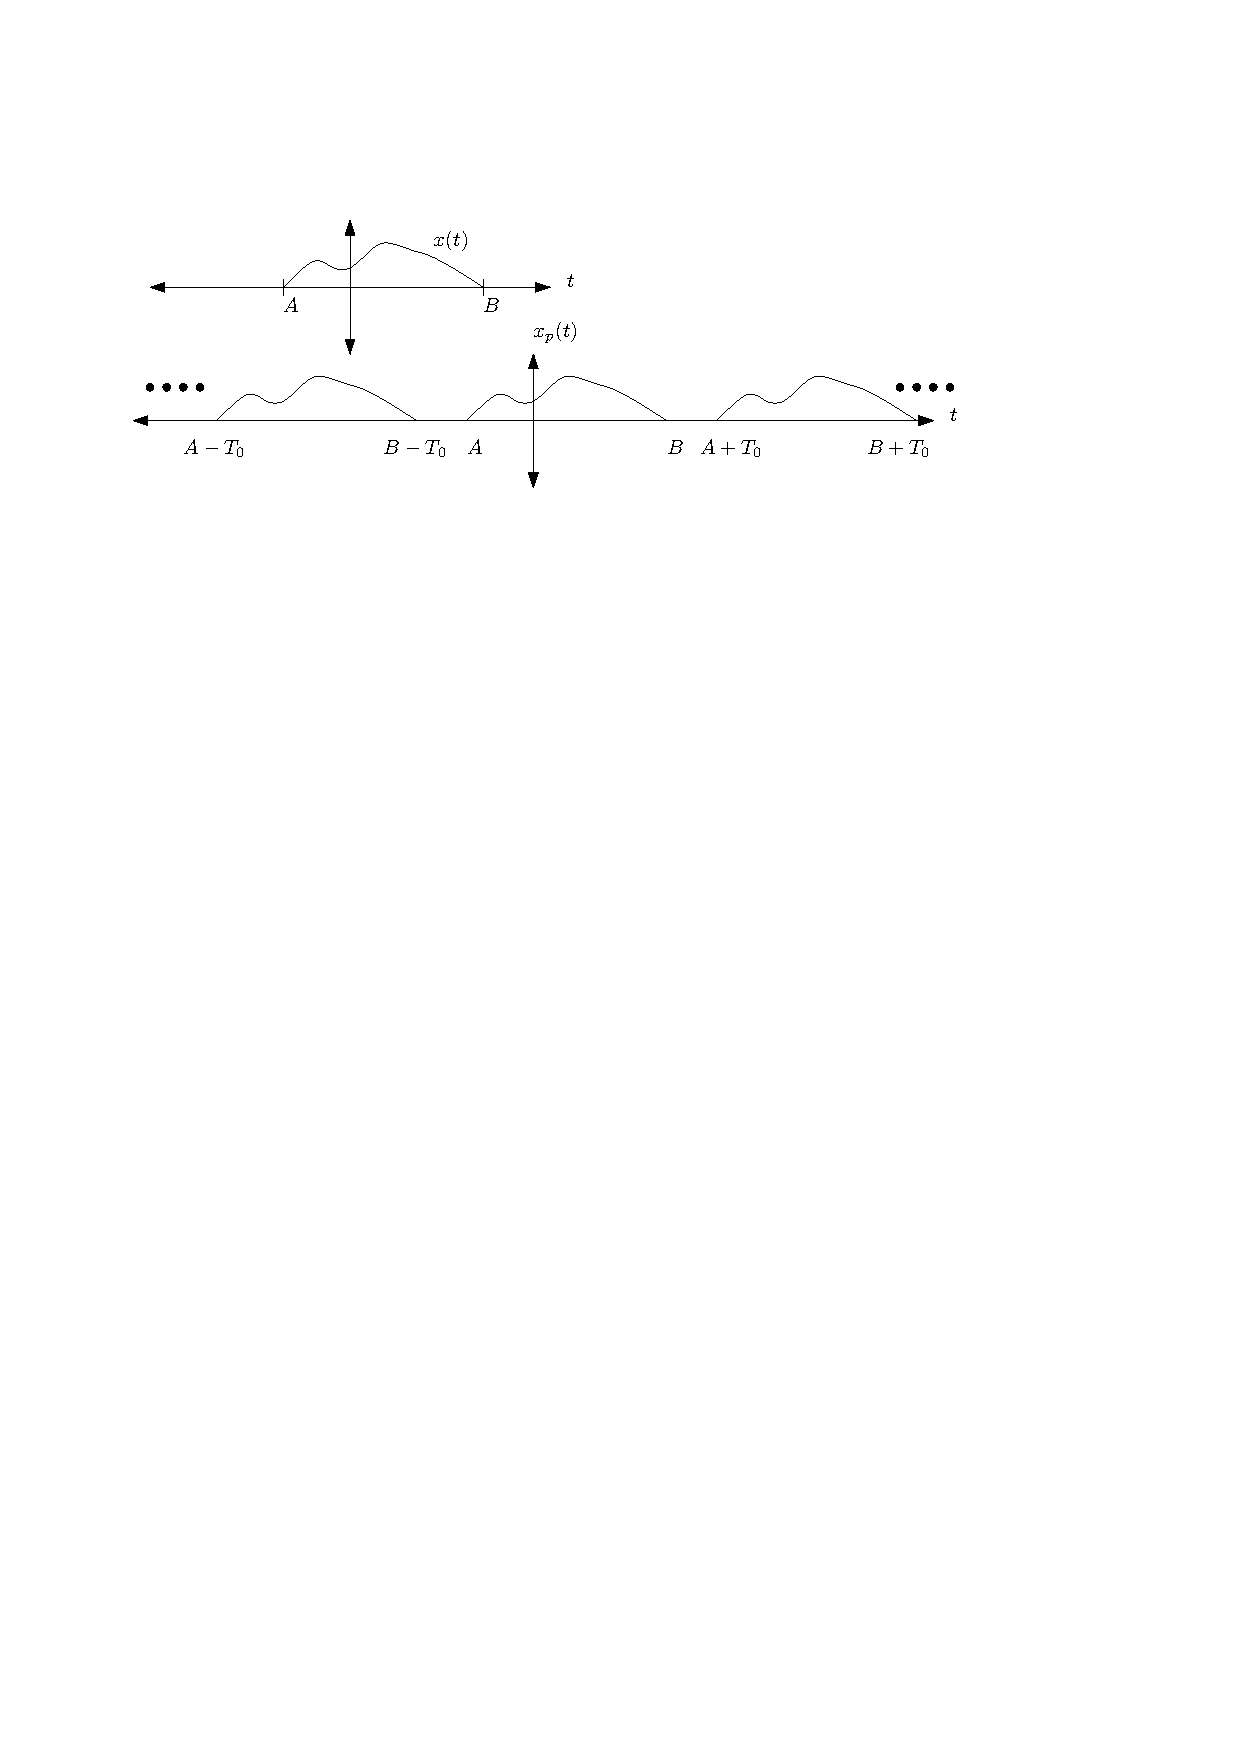
\includegraphics[scale=1]{graphics/ctfs_derivation.pdf}
\end{center}
The CT Fourier series coefficients are
\begin{align*}
  a_k &= \frac{1}{T_0} \int\limits_{T_0} x_p(t) e^{-jk\omega_0 t}\; dt\\
  &= \frac{1}{T_0} \int\limits_{-\infty}^{\infty} x(t) e^{-jk\omega_0 t}\; dt \mbox{ since } x(t) = 0 \mbox{ outside the interval } (A,B)\\
\end{align*}
Define the \emph{CT Fourier Transform} of $x(t)$ as
\[
\boxed{X(\omega) = \int\limits_{-\infty}^{\infty} x(t) e^{-j\omega t}\; dt}
\]
so that
\[
a_k = \frac{1}{T_0} X(k\omega_0)
\]
are samples of $X(\omega)$ spaced at frequencies $\omega_0$. By the CT Fourier series synthesis equation
\[
x(t) = \sum\limits_{k = -\infty}^{\infty} \frac{1}{T_0} X(k\omega_0) e^{jk\omega_0 t} 
\]
Now, let $T_0 \rightarrow \infty$ so that the periodic copies move toward $\infty$ and $x_p(t) \rightarrow x(t)$. At the same time the frequency sample spacing becomes infinitesimal and
\[
X(k\omega_0) e^{jk\omega_0 t} \rightarrow X(\omega) e^{j\omega t}\; d\omega
\]
To give the \emph{Inverse Fourier Transform}
\[
\boxed{x(t) = \frac{1}{2\pi} \int\limits_{-\infty}^{\infty} X(\omega)e^{j\omega t}\; d\omega}
\]
This gives the \emph{Fourier Transform Pair}:
\[
\underbrace{X(\omega) = \mathcal{F}\{x(t)\} = \int\limits_{-\infty}^{\infty} x(t) e^{-j\omega t}\; dt}_{\text{Forward Transform / Analysis Equation}}
\hspace{3em}
\underbrace{x(t) = \mathcal{F}^{-1}\{X(\omega)\} = \frac{1}{2\pi} \int\limits_{-\infty}^{\infty} X(\omega)e^{j\omega t}\; d\omega}_{\text{Inverse Transform / Synthesis Equation}}
\]
The forward transform decomposes $x(t)$ into an infinite number of complex sinusoids. The inverse transform synthesizes a signal as an infinite sum of the sinusoids. It is an example of an \emph{Integral Transform}. Note the signal $x(t)$ and $X(\omega)$ are the same signal, just represented in different \emph{domains}, the time-domain and frequency-domain respectively. 

Similar to the CT Fourier series, the function $X(\omega)$ is called the \emph{spectrum} of the signal $x(t)$. The magnitude spectrum is the function $|X(\omega)|$ and the phase spectrum is the function $\angle X(\omega)$. It is common to plot the spectrum as the combination of the magnitude and phase spectrum.

\begin{example}
  Consider the signal $x(t) = \delta(t)$. The Fourier transform is
  \begin{align*}
    X(\omega) &= \int\limits_{-\infty}^{\infty} x(t) e^{-j\omega t}\; dt\\
    &= \int\limits_{-\infty}^{\infty} \delta(t) e^{-j\omega t}\; dt\\
    &= e^{-j\omega (0)} \mbox{ by the sifting property}\\
    &= 1
  \end{align*}
  $\blacksquare$
\end{example}
\begin{example}
Consider the signal $x(t) = e^{at}u(t)$ for $a\in \mathbb{R}$.  The Fourier transform is
  \begin{align*}
    X(\omega) &= \int\limits_{-\infty}^{\infty} x(t) e^{-j\omega t}\; dt\\
    &= \int\limits_{0}^{\infty}  e^{at} \, e^{-j\omega t}\; dt\\
    &= \int\limits_{0}^{\infty}  e^{(a-j\omega) t}\; dt\\
    &= \frac{1}{a-j\omega } e^{(a-j\omega) t} \Big|_{0}^{\infty}\\
    &= \frac{1}{a-j\omega } \left[ \lim_{T\rightarrow\infty} e^{(a-j\omega) T} - \underbrace{e^{(a-j\omega) (0)}}_{1}\right]
  \end{align*}
  This example raises the question, of when does the Fourier Transform exist? Note if $a < 0$ then the limit above converges to zero, otherwise the integral diverges. In the former case we say the Fourier transform exists, and in the latter that it does not. Thus
  \[
  X(\omega) = \frac{-1}{a-j\omega } = \frac{1}{j\omega-a} \mbox{ for } a < 0\;.
  \]
  Note when $a < 0$, $x(t)$ is an energy signal. A sufficient, but not necessary condition for the Fourier transform to exist is that the signal be an energy signal. For this example, let's examine the spectrum, noting
  \[
  |X(\omega)| = \frac{1}{(a^2 + \omega^2)^\frac{1}{2}} \hspace{2em}\mbox{and}\hspace{2em} \angle X(\omega) = -\arctan\left( \frac{\omega}{-a}\right)
  \]
  plotted below for $a = -1$.
  \begin{center}
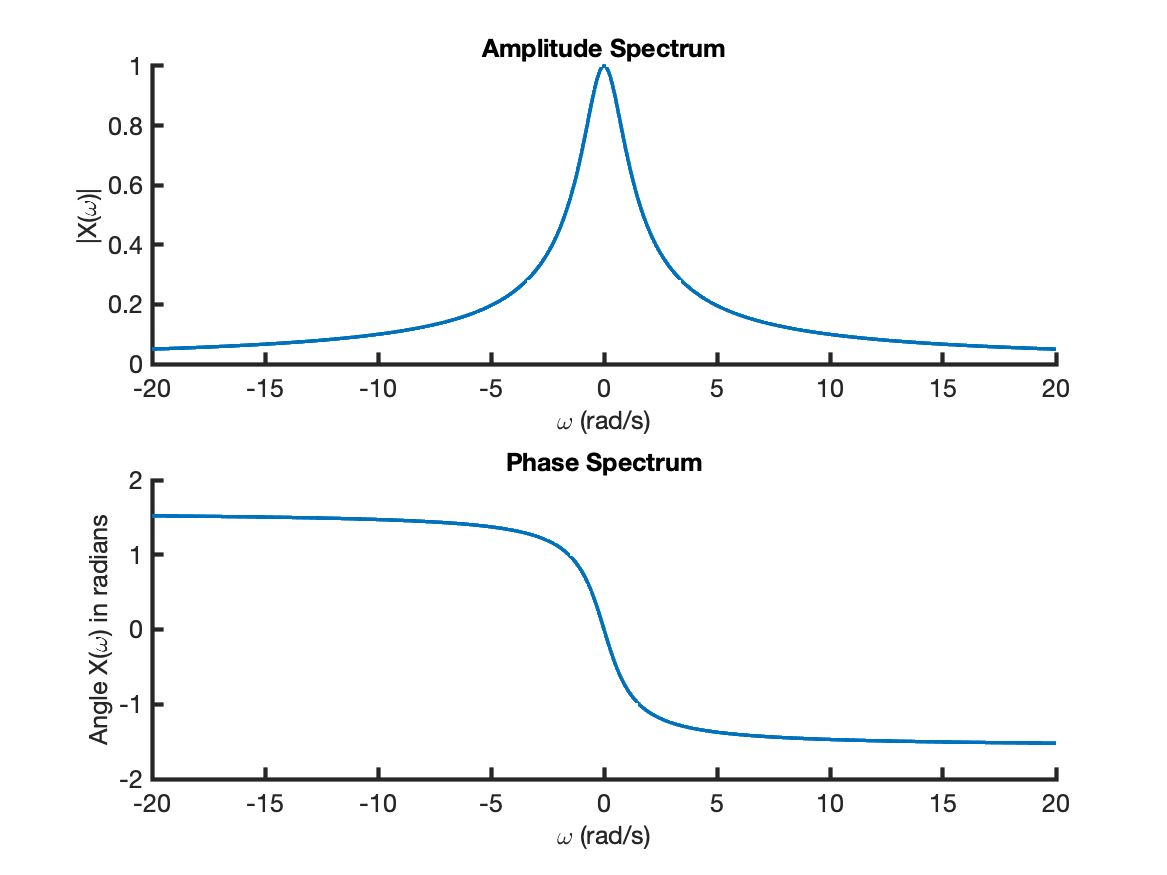
\includegraphics[scale=0.6]{graphics/ctft_example1.png}
  \end{center}
  $\blacksquare$
\end{example}
\begin{example}
Consider the signal $x(t) = e^{j\omega_0 t}$ for $\omega_0\in \mathbb{R}$.  The Fourier transform is
  \begin{align*}
    X(\omega) &= \int\limits_{-\infty}^{\infty} x(t) e^{-j\omega t}\; dt\\
    &= \int\limits_{-\infty}^{\infty}  e^{j\omega_0 t} \, e^{-j\omega t}\; dt\\
    &= \int\limits_{-\infty}^{\infty}  e^{-j(\omega_0-\omega) t}\; dt
  \end{align*}
  For $\omega \neq \omega_0$ this integral evaluates to
  \begin{align*}
    X(\omega) &= \int\limits_{-\infty}^{\infty}  \cos((\omega-\omega_0) t)\; dt + j \int\limits_{-\infty}^{\infty}  \sin((\omega-\omega_0) t)\; dt\\
    &= 0
  \end{align*}
  since the average value of a sinusoid is zero. When $\omega = \omega_0$ this integral diverges
  \[
  \int\limits_{-\infty}^{\infty}  e^{-j(\omega_0-\omega) t}dt = \int\limits_{-\infty}^{\infty}  e^{-j(0) t} dt= \int\limits_{-\infty}^{\infty} dt = \infty 
  \]
  What signal is zero everywhere, but infinite at one point (I am hand-waving a bit here)? The delta function
  \[
  X(\omega) = A\delta(\omega-\omega_0) \mbox{ for some constant } A.
  \]
  To find the constant we can use the inverse transform
  \begin{align*}
    x(t) &= \frac{1}{2\pi} \int\limits_{-\infty}^{\infty} X(\omega)e^{j\omega t}\; d\omega\\
    &= \frac{1}{2\pi} \int\limits_{-\infty}^{\infty}  A\delta(\omega-\omega_0) e^{j\omega t}\; d\omega\\
    &= \frac{1}{2\pi} A e^{j\omega_0 t}\\
    &= e^{j\omega_0 t}
  \end{align*}
  which implies $A = 2\pi$.\\
  $\blacksquare$
\end{example}

\begin{example}
  Consider the signal $x(t) = \cos(\omega_0 t)$ for $\omega_0\in \mathbb{R}$.  The Fourier transform can be found using the result in the previous example by noting
  \begin{align*}
    X(\omega) &= \int\limits_{-\infty}^{\infty} x(t) e^{-j\omega t}\; dt\\
    &= \int\limits_{-\infty}^{\infty}  \cos(\omega_0 t) \, e^{-j\omega t}\; dt\\
    &= \frac{1}{2}\int\limits_{-\infty}^{\infty}   e^{j\omega_0 t} \, e^{-j\omega t}\; dt + \frac{1}{2}\int\limits_{-\infty}^{\infty} e^{-j\omega_0 t} \, e^{-j\omega t}\; dt\\
    &= \frac{1}{2} 2\pi \delta(\omega-\omega_0) + \frac{1}{2} 2\pi \delta(\omega+\omega_0)\\
    &= \pi \delta(\omega-\omega_0) + \pi \delta(\omega+\omega_0)
  \end{align*}
  This example highlights that the cosine signal is composed of exactly two frequencies.\\
  $\blacksquare$
\end{example}

\begin{example}
  Consider the signal
  \[
  X(\omega) = \begin{cases}
    1 & |\omega| < \omega_0\\
    0 & \text{else}
  \end{cases}
  \]
  The Inverse Fourier transform is
  \begin{align*}
    x(t) & = \frac{1}{2\pi} \int\limits_{-\infty}^{\infty} X(\omega)e^{j\omega t}\; d\omega\\
    &= \frac{1}{2\pi} \int\limits_{-\omega_0}^{\omega_0} e^{j\omega t}\; d\omega\\
    &= \frac{1}{2\pi} \frac{1}{jt} \left[ e^{j\omega_0 t} - e^{-j\omega_0 t}\right]\\
    &= \frac{1}{\pi t} \left[ \frac{1}{2j}e^{j\omega_0 t} - \frac{1}{2j} e^{-j\omega_0 t}\right]\\
    &= \frac{1}{\pi t} \sin(\omega_0 t)\\
    &= \frac{\omega_0}{\pi} \frac{\sin(\omega_0 t)}{\omega_0 t}\\
    &= \frac{\omega_0}{\pi} \mbox{sinc}(\omega_0 t)
  \end{align*}
  where $\mbox{sinc}()$ is the (unnormalized) \emph{sinc function}.\\
  $\blacksquare$
\end{example}

\section{Existence of the CT Fourier Transform}

The example of the real exponential above showed that for the Fourier transform to exist, the Fourier (analysis) integral must exist. Similar to the Fourier series some mild conditions, called the Dirichlet conditions, are a sufficient prerequisite for the Fourier transform of a signal $x(t)$ to exist:
\begin{itemize}
\item $x(t)$ is absolutely integrable
  \[
  x(t) = \int\limits_{-\infty}^{\infty} |x(t)|\; dt < \infty
  \]
\item $x(t)$ has a finite number of minima and maxima over any finite interval
\item $x(t)$ has a finite number of finite-valued discontinuities over any finite interval
\end{itemize}

These conditions are not necessary however, and we can extend the Fourier transform to a broader class of signals, if we allow delta functions in the transform, as in the cosine example above. 

\section{Properties of the CT Fourier Transform}

There are several useful properties of the CT Fourier Transform that, when combined with a table of transforms (see Table 4.2, page 329 of OW), allow us to take the Fourier transform of  wide array of signals, and one, the convolution property, that allows us to determine the output of a system in the frequency domain easily. We state these here without proof in rough order of usefulness. See the course text for detailed derivations.

We use the notation $x(t) \stackrel{\mathcal{F}}{\longleftrightarrow} X(\omega)$ to indicate the signals are related by a Fourier Transform pair.
\begin{itemize}
\item Linearity: if $x_1(t) \stackrel{\mathcal{F}}{\longleftrightarrow} X_1(\omega)$ and $x_2(t) \stackrel{\mathcal{F}}{\longleftrightarrow} X_2(\omega)$ then
  \[
  ax_1(t) + bx_2(t) \stackrel{\mathcal{F}}{\longleftrightarrow} aX_1(\omega) + bX_2(\omega)
  \]
\item Convolution: if $x_1(t) \stackrel{\mathcal{F}}{\longleftrightarrow} X_1(\omega)$ and $x_2(t) \stackrel{\mathcal{F}}{\longleftrightarrow} X_2(\omega)$ then
  \[
  x_1(t) * x_2(t) \stackrel{\mathcal{F}}{\longleftrightarrow} X_1(\omega)X_2(\omega)
  \]
  Note in particular if one signal is the system input and the other is the impulse response, the output is the product of the Fourier transforms of each, where the Fourier transform of $h(t)$ is $H(\omega)$, the Eigenvalue or frequency response.
\item Differentiation if $x(t) \stackrel{\mathcal{F}}{\longleftrightarrow} X(\omega)$ then
  \[
  \frac{dx}{dt}(t) \stackrel{\mathcal{F}}{\longleftrightarrow} j\omega X(\omega)
  \]
  This allows us to easily determine the Eigenvalues/Frequency Response from a stable differential equation.
\item Multiplication: if $x_1(t) \stackrel{\mathcal{F}}{\longleftrightarrow} X_1(\omega)$ and $x_2(t) \stackrel{\mathcal{F}}{\longleftrightarrow} X_2(\omega)$ then
  \[
  x_1(t) \cdot x_2(t) \stackrel{\mathcal{F}}{\longleftrightarrow} \frac{1}{2\pi} X_1(\omega)*X_2(\omega)
  \]
  where $X_1(\omega)*X_2(\omega)$ is convolution in the frequency domain
  \[
  X_1(\omega)*X_2(\omega) = \int\limits_{-\infty}^{\infty} X_1(\gamma)*X_2(\omega-\gamma)\;d\gamma 
  \]
\item Time-Shift: if $x(t) \stackrel{\mathcal{F}}{\longleftrightarrow} X(\omega)$ then
  \[
  x(t-t_0) \stackrel{\mathcal{F}}{\longleftrightarrow} X(\omega)e^{-j\omega t_0}
  \]
\item Conjugate Symmetry: if $x(t) \stackrel{\mathcal{F}}{\longleftrightarrow} X(\omega)$ then
  \[
  x^*(t) \stackrel{\mathcal{F}}{\longleftrightarrow} X^*(-\omega)
  \]
  This implies that if $x(t)$ is real, then the magnitude spectrum is an even function, and the phase spectrum is an odd function.

\item Integration: if $x(t) \stackrel{\mathcal{F}}{\longleftrightarrow} X(\omega)$ then
  \[
  \int\limits_{-\infty}^t x(\tau)\; d\tau \stackrel{\mathcal{F}}{\longleftrightarrow} \frac{1}{j\omega} X(\omega) + \pi X(0) \delta(\omega)
  \]
\item Time and Frequency Scaling: if $x(t) \stackrel{\mathcal{F}}{\longleftrightarrow} X(\omega)$ then if $a$ is a real constant
  \[
  x(at) \stackrel{\mathcal{F}}{\longleftrightarrow} \frac{1}{|a|} X\left(\frac{\omega}{a}\right)
  \]
\item Parseval's Relation: if $x(t) \stackrel{\mathcal{F}}{\longleftrightarrow} X(\omega)$ then
  \[
  \int\limits_{0-\infty}^{\infty} |x(t)|^2\; dt =  \frac{1}{2\pi}\int\limits_{0-\infty}^{\infty} |X(\omega)|^2\;d\omega
  \]
\end{itemize}


\section{CT Fourier Transform of a Periodic Signal}

Even though the Fourier transform was derived in the case of an a-periodic signal, the linearity property of the transform, combined with one of our examples above shows us that we can take the Fourier Transform of a periodic signal. Consider a periodic signal with Fourier series expansion
\[
x(t) = \sum\limits_{k = -\infty}^{\infty} a_k e^{jk\omega_0 t}
\]
Taking the Fourier Transform
\[
\mathcal{F}\{x(t)\} = \mathcal{F}\left\{\sum\limits_{k = -\infty}^{\infty} a_k e^{jk\omega_0 t}\right\} = \sum\limits_{k = -\infty}^{\infty} a_k \mathcal{F}\{e^{jk\omega_0 t}\} = \sum\limits_{k = -\infty}^{\infty} a_k 2\pi \delta(\omega-k\omega_0) 
\]
Thus the discrete Fourier series coefficients become the weights of the corresponding delta functions centered at the harmonic frequency.

